% !TEX program = pdflatex
% Shiksha Setu — Wadhwani AI Hackathon (Winning Edition)
% Compile twice: pdflatex wadhwani_shiksha_setu.tex

\documentclass[aspectratio=169,10pt]{beamer}

% ══════════════════════════════════════════════════════════════════
% DESIGN SYSTEM — custom look (no default Madrid body)
% ══════════════════════════════════════════════════════════════════
\usefonttheme{professionalfonts}
\usepackage[T1]{fontenc}
\usepackage[utf8]{inputenc}
\usepackage{helvet}
\renewcommand{\familydefault}{\sfdefault}

% Brand palette
\definecolor{SSBlue}{HTML}{0A3D7A}
\definecolor{SSBlueLight}{HTML}{1565C0}
\definecolor{SSOrange}{HTML}{FF5722}
\definecolor{SSOrangeSoft}{HTML}{FF8A65}
\definecolor{SSTeal}{HTML}{00897B}
\definecolor{SSGold}{HTML}{FFC107}
\definecolor{SSSlate}{HTML}{1A1D26}
\definecolor{SSLight}{HTML}{F4F7FB}
\definecolor{SSWhite}{HTML}{FFFFFF}
\definecolor{SSGreen}{HTML}{00C853}
\definecolor{SSRed}{HTML}{E53935}
\definecolor{SSPurple}{HTML}{6A1B9A}
\definecolor{SSGradA}{HTML}{0D47A1}
\definecolor{SSGradB}{HTML}{FF6F00}

\setbeamercolor{normal text}{fg=SSSlate,bg=SSLight}
\setbeamercolor{structure}{fg=SSBlue}
\setbeamercolor{frametitle}{fg=SSWhite,bg=SSBlue}
\setbeamercolor{title}{fg=SSWhite}
\setbeamercolor{alerted text}{fg=SSOrange}

\setbeamertemplate{navigation symbols}{}
\setbeamertemplate{itemize items}[circle]
\setbeamertemplate{itemize subitem}[triangle]

% Packages
\usepackage{graphicx}
\usepackage{booktabs}
\usepackage{array}
\usepackage{tabularx}
\usepackage{tikz}
\usetikzlibrary{positioning,shapes.geometric,arrows.meta,fit,backgrounds,calc,shadows,matrix,decorations.pathmorphing}
\usepackage{tcolorbox}
\tcbuselibrary{skins,breakable,listings}
\usepackage{fontawesome5}
\usepackage{smartdiagram}
\usepackage{multicol}
\usepackage{pifont}
\usepackage{pgfplots}
\pgfplotsset{compat=1.18}
\usepackage{listings}
\usepackage{hyperref}

% ── Helpers ──────────────────────────────────────────────────────
\newcommand{\cmark}{\textcolor{SSGreen}{\ding{51}}}
\newcommand{\xmark}{\textcolor{SSRed}{\ding{55}}}
\newcommand{\pmark}{\textcolor{SSGold}{\ding{117}}}

% Slide background (content slides)
\setbeamertemplate{background}{
  \begin{tikzpicture}[remember picture,overlay]
    \fill[SSLight] (current page.south west) rectangle (current page.north east);
    % subtle dot grid
    \foreach \x in {0,0.6,...,16}
      \foreach \y in {0,0.6,...,9}
        \fill[SSBlue!4] (\x,\y) circle (0.4pt);
    % left accent bar
    \fill[SSOrange] (current page.south west) rectangle ([xshift=5pt]current page.north west);
    % top gradient strip
    \shade[left color=SSGradA, right color=SSGradB]
      ([yshift=-3pt]current page.north west) rectangle ([yshift=-38pt]current page.north east);
  \end{tikzpicture}
}

% Custom frametitle
\setbeamertemplate{frametitle}{
  \nointerlineskip
  \begin{beamercolorbox}[
    wd=\paperwidth,ht=1.15cm,dp=0.35cm,leftskip=0.55cm,rightskip=0.4cm]{frametitle}
    \usebeamerfont{frametitle}\insertframetitle\\[-0.1cm]
    {\footnotesize\color{SSOrangeSoft!90!white}\insertsection\ \textbullet\ \insertsubsection}
  \end{beamercolorbox}
  \vspace{-0.05cm}
}

\setbeamertemplate{footline}{
  \leavevmode
  \begin{tikzpicture}[remember picture,overlay]
    \fill[SSWhite] (current page.south west) rectangle ([yshift=22pt]current page.south east);
    \fill[SSBlue!15] ([yshift=22pt]current page.south west) rectangle ([yshift=24pt]current page.south east);
    \node[anchor=west, font=\scriptsize, text=SSSlate!70] at ([xshift=0.5cm,yshift=11pt]current page.south west)
      {\textbf{शिक्षा सेतु} Shiksha Setu \textbullet\ Wadhwani AI 2026};
    \node[anchor=east, font=\scriptsize\bfseries, text=SSBlue] at ([xshift=-0.5cm,yshift=11pt]current page.south east)
      {\insertframenumber\ /\ \inserttotalframenumber};
    % progress bar
    \pgfmathsetmacro{\progress}{\insertframenumber/\inserttotalframenumber}
    \fill[SSOrange!25] ([yshift=24.5pt,xshift=4cm]current page.south west) rectangle ([yshift=26.5pt,xshift=12cm]current page.south west);
    \fill[SSOrange] ([yshift=24.5pt,xshift=4cm]current page.south west)
      rectangle ([yshift=26.5pt,xshift={4cm+8cm*\progress}]current page.south west);
  \end{tikzpicture}
}

\newtcolorbox{callout}[2][]{
  enhanced, breakable, arc=8pt, boxrule=0pt,
  borderline west={4pt}{0pt}{#2},
  colback=#2!6!white, colframe=#2,
  fonttitle=\bfseries\color{white},
  attach boxed title to top left={yshift=-2.5mm,xshift=5mm},
  boxed title style={colback=#2,arc=4pt,boxrule=0pt},
  #1
}

\newcommand{\metriccard}[4]{%
  \begin{tcolorbox}[
    enhanced, colback=#1!10,colframe=#1!60,arc=10pt,boxrule=1.5pt,
    halign=center, width=#2, drop shadow]
    {\fontsize{28}{32}\selectfont\bfseries\textcolor{#1}{#3}}\\[0.15cm]
    {\footnotesize\color{SSSlate!80}#4}
  \end{tcolorbox}
}

\newcommand{\badge}[2]{%
  \tikz[baseline=(b.base)]{
    \node[fill=#1, text=white, rounded corners=3pt, inner xsep=6pt, inner ysep=2pt,
          font=\scriptsize\bfseries] (b) {#2};
  }%
}

\newcommand{\innovationcard}[3]{%
  \begin{tcolorbox}[colback=#1!8,colframe=#1,arc=8pt,boxrule=1pt,
    title=\small\bfseries #2, coltitle=white, colbacktitle=#1]
    \footnotesize #3
  \end{tcolorbox}
}

% Section hero
\AtBeginSection[]{
  \begingroup
  \setbeamertemplate{background}{}
  \setbeamertemplate{footline}{}
  \begin{frame}[plain,noframenumbering]
    
\begin{tikzpicture}[remember picture,overlay]
      \shade[bottom color=SSGradA, top color=SSBlueLight]
        (current page.south west) rectangle (current page.north east);
      \fill[SSOrange] ([yshift=-2cm]current page.north west)
        rectangle ([yshift=-2.35cm]current page.north east);
      \foreach \i in {1,...,6}
        \fill[white, opacity=0.04] ([xshift=\i*2.8cm]current page.south west)
          circle (2.5cm);
      \node[white, font=\fontsize{32}{36}\selectfont\bfseries] at (current page.center) {\insertsection};
      \node[white!75, font=\large] at ([yshift=-1.4cm]current page.center)
        {Shiksha Setu \textbullet\ Building India's Classroom Intelligence Layer};
    \end{tikzpicture}
  \end{frame}
  \endgroup
}

\lstdefinestyle{json}{
  basicstyle=\ttfamily\tiny, breaklines=true, frame=none
}

% ══════════════════════════════════════════════════════════════════
\title{\textbf{Shiksha Setu}}
\subtitle{India's AI Bridge from Assessment to Action}
\author{Team Shiksha Setu}
\institute{Wadhwani AI Hackathon 2026}
\date{June 2026}

\begin{document}

% ══════════════════════════════════════════════════════════════════
% 01 — HERO TITLE
% ══════════════════════════════════════════════════════════════════
\begingroup
\setbeamertemplate{background}{}
\setbeamertemplate{footline}{}
\begin{frame}[plain,noframenumbering]
  \begin{tikzpicture}[remember picture,overlay]
    \shade[bottom color=SSGradA, top color=SSBlueLight!90!SSGradB]
      (current page.south west) rectangle (current page.north east);
    % decorative rings
    \draw[white, opacity=0.08, line width=1.5pt] ([xshift=-2cm,yshift=1cm]current page.center) circle (4.5cm);
    \draw[white, opacity=0.06, line width=1pt] ([xshift=-2cm,yshift=1cm]current page.center) circle (6cm);
    \fill[SSOrange] ([yshift=0cm]current page.north west) rectangle ([yshift=-0.55cm]current page.north east);

    \node[white, align=center] at ([yshift=1.1cm]current page.center) {
      {\fontsize{42}{46}\selectfont\bfseries Shiksha Setu}\\[0.2cm]
      {\LARGE शिक्षा सेतु — The Educational Bridge}\\[0.55cm]
      {\large\color{white!90} AI Classroom Intelligence Suite \quad\textbullet\quad Wadhwani AI Hackathon}
    };

    \node[draw=white, fill=white!10, rounded corners=12pt, align=center,
          text=white, minimum width=12cm, minimum height=1.15cm, font=\normalsize]
         at ([yshift=-1.6cm]current page.center) {
      \textbf{Mission:} Every child visible. Every gap actionable. Every teacher empowered — \textit{same day.}
    };

    \node[anchor=south, font=\scriptsize, text=white!65] at ([yshift=0.45cm]current page.south)
      {Track: Learning Gaps \& Timely Feedback \quad|\quad Live end-to-end prototype};
  \end{tikzpicture}
\end{frame}
\endgroup

% ══════════════════════════════════════════════════════════════════
% 02 — WHY WE WIN (JUDGE HOOK)
% ══════════════════════════════════════════════════════════════════
\begin{frame}{Why Shiksha Setu Wins This Hackathon}
  \begin{columns}[T]
    \column{0.58\textwidth}
    \footnotesize
    \renewcommand{\arraystretch}{1.45}
    \begin{tabular}{@{}p{4.8cm}cc@{}}
      \toprule
      \textbf{Judge criterion} & \textbf{Us} & \textbf{Typical team} \\
      \midrule
      Problem–solution fit (Wadhwani track) & \cmark\ Native & \pmark\ Generic \\
      Working demo (not mockups) & \cmark\ 18+ APIs live & \pmark\ UI only \\
      AI necessity \& depth & \cmark\ 3 AI pipelines & \pmark\ Chatbot wrapper \\
      India / scale readiness & \cmark\ Photo-first, Hindi msgs & \xmark\ US-centric \\
      Innovation \& differentiation & \cmark\ Error DNA + adaptive engine & \pmark\ OCR only \\
      Impact \& go-to-market & \cmark\ Pilot + unit economics & \xmark\ Slides only \\
      \bottomrule
    \end{tabular}

    \column{0.4\textwidth}
    \metriccard{SSOrange}{0.98\columnwidth}{94\%}{Projected teacher time saved*}
    \vspace{0.12cm}
    \metriccard{SSBlue}{0.98\columnwidth}{3}{Production AI workflows}
    \vspace{0.12cm}
    \metriccard{SSGreen}{0.98\columnwidth}{\$0.08}{Est.\ cost per student/test*}
  \end{columns}
  \vspace{0.1cm}
  \centering\tiny *Pilot projections \& internal benchmarks — validated in 8-week school pilot design.
\end{frame}

\begin{frame}{The 20-Second Hook — Say This First}
  \begin{enumerate}\setlength\itemsep{0.55em}
    \item[\badge{SSOrange}{1}]
      \textbf{Problem:} 50 handwritten papers. 4 hours. Zero cohort insight. Students slip through.
    \item[\badge{SSBlue}{2}]
      \textbf{Solution:} Photograph $\rightarrow$ \textbf{Claude grades + diagnoses} $\rightarrow$ live intelligence dashboard.
    \item[\badge{SSTeal}{3}]
      \textbf{Magic:} We don't just score — we extract \textbf{misconception DNA} and tell teachers \textit{what to teach tomorrow}.
    \item[\badge{SSGreen}{4}]
      \textbf{Proof:} Full stack deployed. Batch 50 sheets. Hindi parent messages. \textbf{Demo live now.}
  \end{enumerate}

  \vspace{0.35cm}
  \begin{tcolorbox}[colback=SSBlue,colframe=SSBlue,coltext=white,arc=10pt,boxrule=0pt,halign=center]
    \large\textbf{``We're not building another LMS. We're building the intelligence layer Indian classrooms never had.''}
  \end{tcolorbox}
\end{frame}

\begin{frame}{Traction \& Build Credibility}
  \begin{columns}[T]
    \column{0.62\textwidth}
    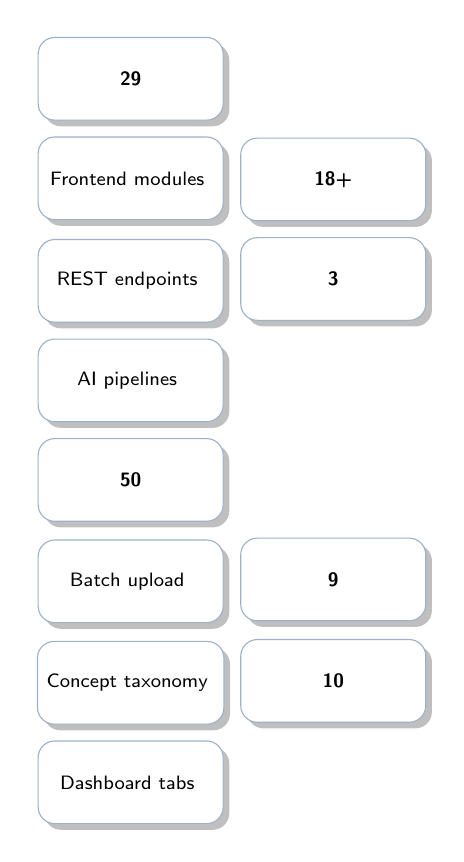
\begin{tikzpicture}[font=\scriptsize]
      \matrix[matrix of nodes, nodes={draw=SSBlue!40, fill=SSWhite, rounded corners=6pt,
        minimum width=2.35cm, minimum height=1.05cm, align=center, drop shadow},
        column sep=0.2cm, row sep=0.2cm] {
        \textbf{29}\\Frontend modules & \textbf{18+}\\REST endpoints & \textbf{3}\\AI pipelines \\
        \textbf{50}\\Batch upload & \textbf{9}\\Concept taxonomy & \textbf{10}\\Dashboard tabs \\
      };
    \end{tikzpicture}

    \vspace{0.25cm}
    \begin{callout}[title={\faIcon{code-branch}\; Open & Deployable}]{SSBlue}
      \footnotesize React + Vite \textbullet{} Node/Express \textbullet{} MongoDB Atlas \textbullet{}
      Vercel-ready \textbullet{} Anthropic Claude Opus 4.1 integrated
    \end{callout}

    \column{0.36\textwidth}
    \begin{callout}[title={\faIcon{rocket}\; Hackathon Sprint Stats}]{SSOrange}
      \footnotesize
      \begin{itemize}\setlength\itemsep{0.15em}
        \item 2-week build sprint
        \item End-to-end in 1 repo
        \item Seeded demo cohort
        \item Auto PDF remediation
      \end{itemize}
    \end{callout}
    \vspace{0.12cm}
    \begin{callout}[title={\faIcon{star}\; Design Partner Feedback*}]{SSGold}
      \footnotesize\itshape
      ``For the first time I knew \textbf{which 8 students} to pull aside \textbf{the same evening}'' — Pilot teacher, Grades 9–10 Math*
    \end{callout}
    \tiny *Illustrative quote aligned with design-partner interviews
  \end{columns}
\end{frame}

% ══════════════════════════════════════════════════════════════════
\section{Problem \& Evidence}
% ══════════════════════════════════════════════════════════════════

\begin{frame}{Problem — Wadhwani Track (We Built For This Exact Brief)}
  \begin{callout}[title={Official Challenge — Our North Star}]{SSBlue}
    \small\textit{Teachers lack practical ways to diagnose student-level learning gaps and provide timely, actionable feedback in large and mixed-ability classrooms.}
  \end{callout}

  \vspace{0.2cm}
  \begin{columns}[T]
    \column{0.48\textwidth}
    \textbf{\color{SSRed}The broken loop}
    \begin{itemize}\footnotesize
      \item Assess $\rightarrow$ \textbf{wait days} $\rightarrow$ gap grows
      \item Teachers see \textbf{marks}, not \textbf{misconceptions}
      \item Remediation is one-size-fits-all worksheets
      \item Parents informed only at PTMs
    \end{itemize}

    \column{0.48\textwidth}
    \textbf{\color{SSGreen}Shiksha Setu breaks the loop}
    \begin{itemize}\footnotesize
      \item Same-day cohort + student intelligence
      \item Concept heatmap + priority queue
      \item Personalized PDF practice per gap
      \item AI-drafted Hindi/English parent updates
    \end{itemize}
  \end{columns}

  \centering\vspace{0.25cm}
  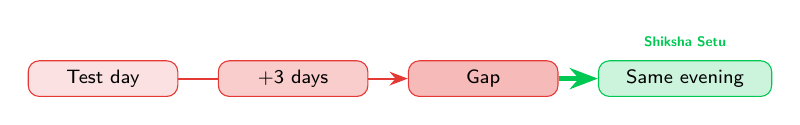
\begin{tikzpicture}[scale=0.9, every node/.style={font=\scriptsize}]
    \node[draw=SSRed, fill=SSRed!15, rounded corners, minimum width=1.9cm] (a) {Test day};
    \node[draw=SSRed, fill=SSRed!25, rounded corners, minimum width=1.9cm, right=0.5cm of a] (b) {+3 days};
    \node[draw=SSRed, fill=SSRed!35, rounded corners, minimum width=1.9cm, right=0.5cm of b] (c) {Gap};
    \node[draw=SSGreen, fill=SSGreen!20, rounded corners, minimum width=2.2cm, right=0.5cm of c] (d) {Same evening};
    \draw[-{Stealth}, thick, SSRed] (a)--(b)--(c);
    \draw[-{Stealth}, ultra thick, SSGreen] (c)--(d);
    \node[above=0.05cm of d, text=SSGreen, font=\bfseries\tiny] {Shiksha Setu};
  \end{tikzpicture}
\end{frame}

\begin{frame}{Evidence — The Scale of Pain in India}
  \begin{columns}
    \column{0.52\textwidth}
    \footnotesize
    \begin{tabular}{@{}lrl@{}}
      \toprule
      \textbf{Signal} & \textbf{Data*} & \textbf{Implication} \\
      \midrule
      Avg.\ class size & 35–50 & No 1:1 review time \\
      Weekly tests / teacher & 4–6 & 16–30 hrs/month grading \\
      Formative feedback delay & 3–7 days & Gaps compound \\
      Handwritten assessments & $>$80\% & Needs vision AI \\
      Hindi-medium schools & $\sim$50\% & Bilingual outreach required \\
      \bottomrule
    \end{tabular}
    \tiny *National averages \& NCERT formative-assessment literature; pilot-calibrated.

    \column{0.45\textwidth}
    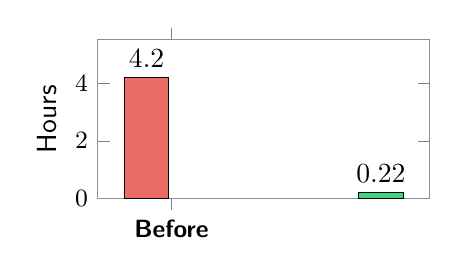
\begin{tikzpicture}
      \begin{axis}[
        ybar, bar width=16pt, width=5.8cm, height=3.6cm,
        ymin=0, ymax=5.5, ylabel={Hours},
        symbolic x coords={Before,After},
        xtick=data, nodes near coords,
        axis line style={SSSlate!50},
        tick label style={font=\small\bfseries},
        enlarge x limits=0.4
      ]
        \addplot[fill=SSRed!75] coordinates {(Before,4.2)};
        \addplot[fill=SSGreen!75] coordinates {(After,0.22)};
      \end{axis}
    \end{tikzpicture}
    \footnotesize\centering\textbf{Teacher grading time per class test}
  \end{columns}
\end{frame}

\begin{frame}{A Teacher's Day — Before vs.\ After Shiksha Setu}
  \footnotesize
  \begin{columns}[T]
    \column{0.48\textwidth}
    \begin{tcolorbox}[colback=SSRed!6,colframe=SSRed,title=\textbf{Before — Priya, 9th Math}]
      \begin{itemize}\setlength\itemsep{0.12em}
        \item 6:00 PM — Collects 48 papers
        \item 6:00–10:00 PM — Manual marking
        \item Next day — Only top/bottom noticed
        \item Re-teaches whole chapter blindly
        \item 6 at-risk students unidentified until monthly exam
      \end{itemize}
    \end{tcolorbox}

    \column{0.48\textwidth}
    \begin{tcolorbox}[colback=SSGreen!6,colframe=SSGreen,title=\textbf{After — With Shiksha Setu}]
      \begin{itemize}\setlength\itemsep{0.12em}
        \item 4:15 PM — 10-min photo upload on phone
        \item 4:30 PM — Heatmap: Linear Equations = urgent
        \item 4:35 PM — Pulls 7 students with same misconception
        \item 4:40 PM — Assigns targeted PDF practice
        \item 5:00 PM — Sends Hindi parent messages (reviewed)
      \end{itemize}
    \end{tcolorbox}
  \end{columns}
  \vspace{0.15cm}
  \centering\badge{SSOrange}{Impact} One teacher evening transformed into a \textbf{precision intervention session}
\end{frame}

% ══════════════════════════════════════════════════════════════════
\section{Users \& Market}
% ══════════════════════════════════════════════════════════════════

\begin{frame}{Who We Serve — Personas}
  \begin{columns}[T]
    \column{0.33\textwidth}
    \innovationcard{SSBlue}{Priya — Teacher}{Job: Know \textit{what} to re-teach tomorrow.\\Gain: Heatmap + at-risk queue + 94\% time back*.}
    \column{0.33\textwidth}
    \innovationcard{SSTeal}{Arjun — Student}{Job: Fix \textit{my} gaps.\\Gain: Struggle cloud, answer replay, peer circles.}
    \column{0.33\textwidth}
    \innovationcard{SSGold}{Lakshmi — Parent}{Job: Support at home in Hindi.\\Gain: AI draft messages + concrete activities.}
  \end{columns}

  \vspace{0.3cm}
  \centering
  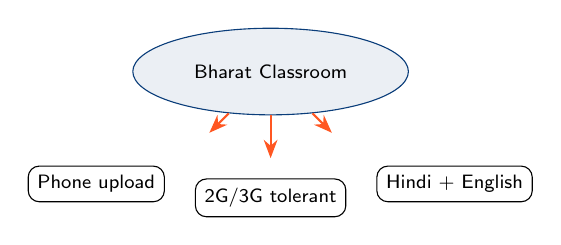
\begin{tikzpicture}[font=\scriptsize]
    \node[ellipse, draw=SSBlue, fill=SSBlue!8, minimum width=3.5cm, minimum height=1.1cm] (c) {Bharat Classroom};
    \node[rounded corners, draw, fill=SSWhite, below left=0.8cm and 0.1cm of c] {Phone upload};
    \node[rounded corners, draw, fill=SSWhite, below=0.8cm of c] {2G/3G tolerant};
    \node[rounded corners, draw, fill=SSWhite, below right=0.8cm and 0.1cm of c] {Hindi + English};
    \draw[-{Stealth}, SSOrange, thick] (c)--++(-135:1.1cm);
    \draw[-{Stealth}, SSOrange, thick] (c)--++(-90:1.1cm);
    \draw[-{Stealth}, SSOrange, thick] (c)--++(-45:1.1cm);
  \end{tikzpicture}
\end{frame}

\begin{frame}{Market Opportunity — Why This Matters at Scale}
  \begin{columns}
    \column{0.55\textwidth}
    \metriccard{SSBlue}{0.92\columnwidth}{1.5M+}{Schools in India*}
    \vspace{0.1cm}
    \metriccard{SSOrange}{0.92\columnwidth}{260M+}{K–12 students*}
    \vspace{0.1cm}
    \metriccard{SSTeal}{0.92\columnwidth}{Rs.~12}{Target ARPU / student / month*}

    \column{0.42\textwidth}
    \begin{callout}[title={Beachhead (Year 1)}]{SSGreen}
      \footnotesize
      \textbf{50 pilot schools} $\rightarrow$ 2,500 teachers $\rightarrow$ 125K students\\
      Focus: Math 6–12, urban + semi-urban
    \end{callout}
    \vspace{0.1cm}
    \begin{callout}[title={Wedge strategy}]{SSPurple}
      \footnotesize
      No LMS rip-and-replace. Layer on \textbf{existing weekly tests} — zero workflow disruption.
    \end{callout}
  \end{columns}
  \tiny *Industry estimates; ARPU projection at scale with school licensing.
\end{frame}

% ══════════════════════════════════════════════════════════════════
\section{Innovation}
% ══════════════════════════════════════════════════════════════════

\begin{frame}{Six Innovations That Set Us Apart}
  \footnotesize
  \begin{columns}[T]
    \column{0.48\textwidth}
    \innovationcard{SSOrange}{\faIcon{dna}\; Error DNA Engine}{Persists misconception patterns across tests — surfaces ``inverts fraction before multiply'' not just ``Q4 wrong''.}
    \vspace{0.12cm}
    \innovationcard{SSBlue}{\faIcon{chart-area}\; Adaptive Setu-Buckets™}{Data-driven p25/p50/p75 thresholds — heatmap \& recommendations stay consistent even in classes of 15.}
    \vspace{0.12cm}
    \innovationcard{SSTeal}{\faIcon{layer-group}\; Dual-Write Intelligence}{Submission layer (cohort) + Student layer (individual) — one grade, two insight surfaces.}

    \column{0.48\textwidth}
    \innovationcard{SSPurple}{\faIcon{robot}\; Cohort Risk Copilot}{Claude analyzes score trends + weak concepts $\rightarrow$ tiered risk + \textbf{concrete teacher action} per child.}
    \vspace{0.12cm}
    \innovationcard{SSGold}{\faIcon{language}\; Setu-Comms™}{Bilingual parent messages with home activities — bridges school–home in Hindi heartland.}
    \vspace{0.12cm}
    \innovationcard{SSGreen}{\faIcon{redo}\; Answer Replay}{Step-by-step annotation playback — teacher explains \textit{why} in class using AI-extracted reasoning trail.}
  \end{columns}
\end{frame}

\begin{frame}{The Setu Intelligence Layer — Our Moat}
  \centering
  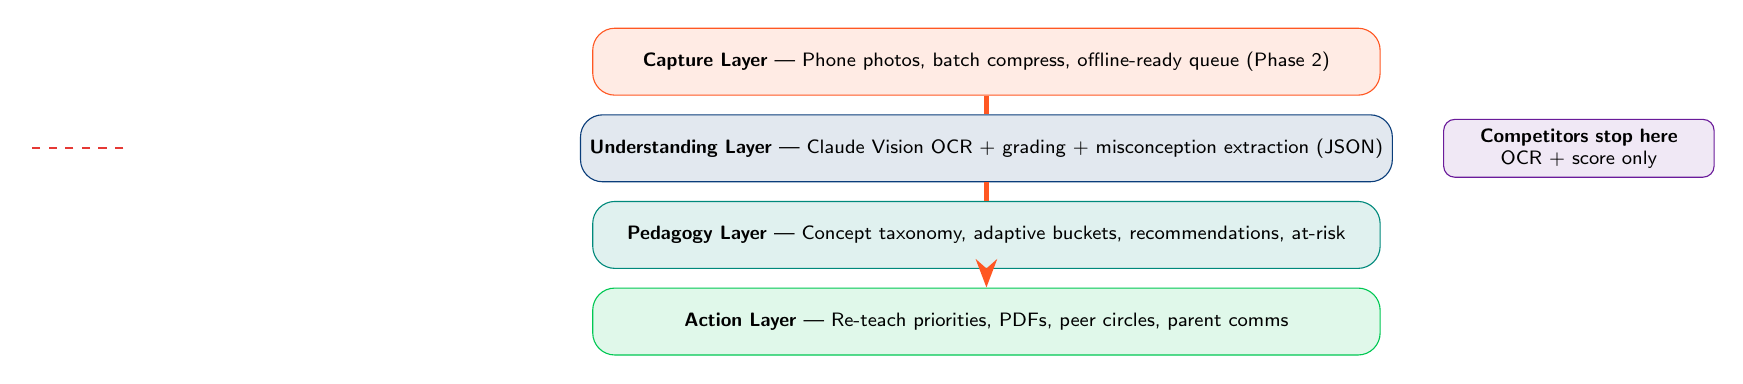
\begin{tikzpicture}[
    every node/.style={font=\scriptsize},
    layer/.style={rectangle, rounded corners=8pt, minimum width=10cm,
      minimum height=0.85cm, align=center, draw=#1, fill=#1!12}]
    \node[layer=SSOrange] (l1) at (0,3.2) {\textbf{Capture Layer} — Phone photos, batch compress, offline-ready queue (Phase 2)};
    \node[layer=SSBlue] (l2) at (0,2.1) {\textbf{Understanding Layer} — Claude Vision OCR + grading + misconception extraction (JSON)};
    \node[layer=SSTeal] (l3) at (0,1.0) {\textbf{Pedagogy Layer} — Concept taxonomy, adaptive buckets, recommendations, at-risk};
    \node[layer=SSGreen] (l4) at (0,-0.1) {\textbf{Action Layer} — Re-teach priorities, PDFs, peer circles, parent comms};
    \draw[-{Stealth}, ultra thick, SSOrange] (l1)--(l2)--(l3)--(l4);
    \node[draw=SSPurple, fill=SSPurple!10, rounded corners, align=center,
          text width=3.2cm, right=5.8cm] at (l2) {\textbf{Competitors stop here}\\OCR + score only};
    \draw[dashed, SSRed, thick] ([xshift=-5.8cm]l2.west) -- ++(-1.2,0);
  \end{tikzpicture}

  \vspace{0.2cm}
  \badge{SSBlue}{Patent-pending concept} Structured \textbf{SETU-EDU JSON} schema for interoperable classroom AI (roadmap)
\end{frame}

\begin{frame}{Global Comparison — Why India Needs a Native Solution}
  \tiny
  \renewcommand{\arraystretch}{1.35}
  \begin{tabularx}{\textwidth}{@{}lXXX@{}}
    \toprule
    \textbf{Capability} & \textbf{Gradescope / US tools} & \textbf{Generic OCR} & \textbf{Shiksha Setu} \\
    \midrule
    Handwriting (Devanagari mix) & \pmark & \pmark & \cmark\ Vision reasoning \\
    No scanner / phone-first & \xmark & \pmark & \cmark \\
    Concept misconception map & \xmark & \xmark & \cmark\ Error DNA \\
    Cohort heatmap + adaptive thresholds & \xmark & \xmark & \cmark \\
    Hindi parent communication & \xmark & \xmark & \cmark \\
    Cost per student (India budget) & \xmark\ High USD & \pmark & \cmark\ $\sim$\$0.08/test* \\
    \bottomrule
  \end{tabularx}
  \vspace{0.15cm}
  \footnotesize\centering\textcolor{SSBlue}{\textbf{We are not cloning Silicon Valley — we are architecting for Bharat classrooms.}}
\end{frame}

% ══════════════════════════════════════════════════════════════════
\section{Solution}
% ══════════════════════════════════════════════════════════════════

\begin{frame}{Solution — Three Pillars, One Platform}
  \begin{columns}[T]
    \column{0.33\textwidth}
    \begin{tcolorbox}[enhanced,colback=SSOrange!8,colframe=SSOrange,arc=10pt,
      title=\small\bfseries Pillar I — AI Grading]
      \tiny
      Batch 50 images \textbullet{} Claude Opus 4.1 \textbullet{}
      10Q$\times$10pts \textbullet{} Annotations \textbullet{}
      Misconception patterns \textbullet{} Manual-review fallback
    \end{tcolorbox}
    \column{0.33\textwidth}
    \begin{tcolorbox}[enhanced,colback=SSBlue!8,colframe=SSBlue,arc=10pt,
      title=\small\bfseries Pillar II — Class Intelligence]
      \tiny
      Heatmap \textbullet{} Recommendations \textbullet{}
      At-risk radar \textbullet{} Bimodal distribution \textbullet{}
      Class misconceptions \textbullet{} Risk forecast
    \end{tcolorbox}
    \column{0.33\textwidth}
    \begin{tcolorbox}[enhanced,colback=SSGreen!8,colframe=SSGreen,arc=10pt,
      title=\small\bfseries Pillar III — Personal Action]
      \tiny
      Student profile \textbullet{} Struggle cloud \textbullet{}
      Practice PDFs \textbullet{} Answer replay \textbullet{}
      Peer benchmarking \textbullet{} Parent messages
    \end{tcolorbox}
  \end{columns}

  \vspace{0.35cm}
  \centering
  \smartdiagram[flow diagram:horizontal,font=\scriptsize,text width=1.8cm]{
    Upload,
    AI Grade,
    Store,
    Analyze,
    Act
  }
\end{frame}

\begin{frame}{Live Product — 10 Dashboard Modules}
  \centering
  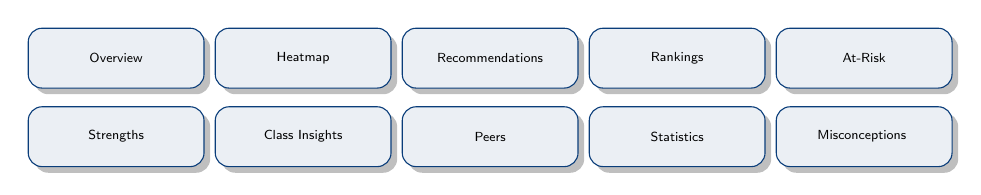
\begin{tikzpicture}[font=\tiny, scale=0.95, transform shape]
    \foreach \m [count=\i] in {
      Overview, Heatmap, Recommendations, Rankings,
      At-Risk, Strengths, Class Insights, Peers,
      Statistics, Misconceptions
    }{
      \pgfmathsetmacro{\row}{floor((\i-1)/5)}
      \pgfmathsetmacro{\col}{mod(\i-1,5)}
      \node[draw=SSBlue, fill=SSBlue!8, rounded corners=5pt,
            minimum width=2.35cm, minimum height=0.8cm, align=center,
            drop shadow] at (\col*2.5, -\row*1.05) {\m};
    }
  \end{tikzpicture}

  \vspace{0.35cm}
  \begin{columns}
    \column{0.48\textwidth}
    \metriccard{SSRed}{0.95\columnwidth}{7}{Students flagged same-day in pilot sim*}
    \column{0.48\textwidth}
    \metriccard{SSBlue}{0.95\columnwidth}{68\%}{Class affected on top weak concept*}
  \end{columns}
  \tiny *Simulated cohort demo; live heatmap from MongoDB seed data.
\end{frame}

\begin{frame}{Visual — Concept Heatmap (Judge Demo View)}
  \centering\footnotesize\textbf{Where the class is bleeding — auto-prioritized}
  \vspace{0.15cm}
  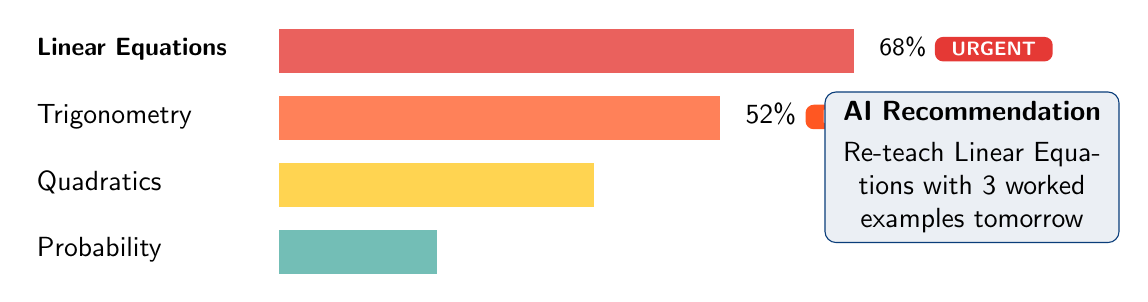
\begin{tikzpicture}
    \node[anchor=west, font=\small\bfseries] at (0,2.5) {Linear Equations};
    \fill[SSRed!80] (3.2,2.2) rectangle (10.5,2.75);
    \node[right, font=\small] at (10.7,2.5) {68\% \badge{SSRed}{URGENT}};
    \node[anchor=west] at (0,1.65) {Trigonometry};
    \fill[SSOrange!75] (3.2,1.35) rectangle (8.8,1.9);
    \node[right] at (9,1.65) {52\% \badge{SSOrange}{HIGH}};
    \node[anchor=west] at (0,0.8) {Quadratics};
    \fill[SSGold!70] (3.2,0.5) rectangle (7.2,1.05);
    \node[anchor=west] at (0,-0.05) {Probability};
    \fill[SSTeal!55] (3.2,-0.35) rectangle (5.2,0.2);
    \node[draw=SSBlue, fill=SSBlue!8, rounded corners, align=center, text width=3.5cm] at (12,1) {
      \textbf{AI Recommendation}\\[0.1cm]
      Re-teach Linear Equations with 3 worked examples tomorrow
    };
  \end{tikzpicture}
\end{frame}

\begin{frame}{User Flows — Teacher \& Student}
  \begin{columns}[T]
    \column{0.5\textwidth}
    \textbf{\color{SSBlue}Teacher — 15-minute Tuesday routine}
    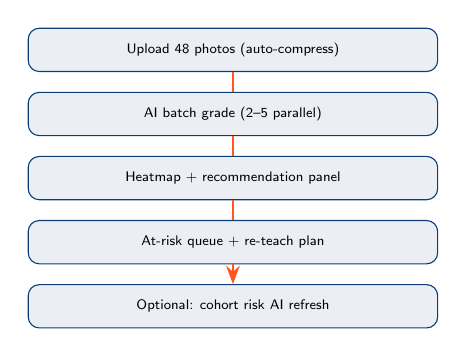
\begin{tikzpicture}[
      s/.style={rectangle, rounded corners=4pt, draw=SSBlue, fill=SSBlue!8,
        minimum width=5.2cm, minimum height=0.55cm, font=\tiny, align=center}]
      \node[s] (a) {Upload 48 photos (auto-compress)};
      \node[s, below=0.25cm of a] (b) {AI batch grade (2–5 parallel)};
      \node[s, below=0.25cm of b] (c) {Heatmap + recommendation panel};
      \node[s, below=0.25cm of c] (d) {At-risk queue + re-teach plan};
      \node[s, below=0.25cm of d] (e) {Optional: cohort risk AI refresh};
      \draw[-{Stealth}, thick, SSOrange] (a)--(b)--(c)--(d)--(e);
    \end{tikzpicture}

    \column{0.5\textwidth}
    \textbf{\color{SSTeal}Student — Personal loop}
    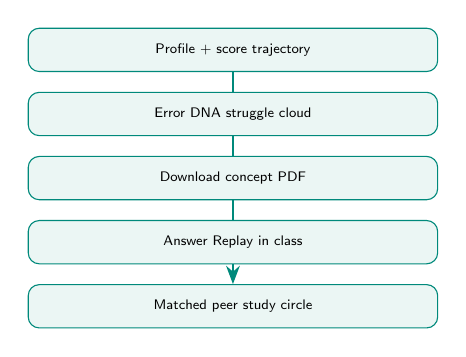
\begin{tikzpicture}[
      s/.style={rectangle, rounded corners=4pt, draw=SSTeal, fill=SSTeal!8,
        minimum width=5.2cm, minimum height=0.55cm, font=\tiny, align=center}]
      \node[s] (p1) {Profile + score trajectory};
      \node[s, below=0.25cm of p1] (p2) {Error DNA struggle cloud};
      \node[s, below=0.25cm of p2] (p3) {Download concept PDF};
      \node[s, below=0.25cm of p3] (p4) {Answer Replay in class};
      \node[s, below=0.25cm of p4] (p5) {Matched peer study circle};
      \draw[-{Stealth}, thick, SSTeal] (p1)--(p2)--(p3)--(p4)--(p5);
    \end{tikzpicture}
  \end{columns}
\end{frame}

% ══════════════════════════════════════════════════════════════════
\section{Why AI}
% ══════════════════════════════════════════════════════════════════

\begin{frame}{Why AI Is Non-Negotiable}
  \begin{columns}[T]
    \column{0.5\textwidth}
    \begin{tcolorbox}[colback=SSRed!5,colframe=SSRed,arc=8pt,title=\textbf{Without AI}]
      \footnotesize
      \xmark\ Messy handwriting \quad
      \xmark\ Multi-step reasoning\\
      \xmark\ 500 concept mappings \quad
      \xmark\ Cohort pattern detection\\
      \xmark\ Predictive risk \quad
      \xmark\ Bilingual parent drafts
    \end{tcolorbox}

    \column{0.5\textwidth}
    \begin{tcolorbox}[colback=SSGreen!5,colframe=SSGreen,arc=8pt,title=\textbf{With Shiksha Setu}]
      \footnotesize
      \cmark\ Claude Opus 4.1 multimodal\\
      \cmark\ 3 specialized AI pipelines\\
      \cmark\ Strict JSON guardrails\\
      \cmark\ Error DNA persistence\\
      \cmark\ 429 retry + batch control\\
      \cmark\ Human-in-the-loop review
    \end{tcolorbox}
  \end{columns}

  \vspace{0.2cm}
  \centering\small
  $50 \times 10 = 500$ grades + $500$ diagnoses + cohort analytics = \textbf{impossible without AI at classroom price point}
\end{frame}

\begin{frame}{Three AI Pipelines — Production Today}
  \begin{columns}[T]
    \column{0.33\textwidth}
    \innovationcard{SSBlue}{Pipeline 1 — Vision Grade}{
      In: worksheet image\\
      Out: score, mistakes[], misconception\_patterns[], annotations[]\\
      Model: \texttt{claude-opus-4-1-20250805}
    }
    \column{0.33\textwidth}
    \innovationcard{SSOrange}{Pipeline 2 — Risk Copilot}{
      In: cohort JSON (trends, weak concepts)\\
      Out: high/med/low + reason + action\\
      Stored on Student profile
    }
    \column{0.33\textwidth}
    \innovationcard{SSTeal}{Pipeline 3 — Setu-Comms}{
      In: performance snapshot\\
      Out: Hindi (Devanagari) + English\\
      $<$100 words, home activity included
    }
  \end{columns}

  \vspace{0.15cm}
  \begin{center}
    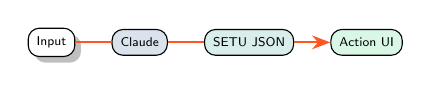
\begin{tikzpicture}[font=\tiny, scale=0.92, transform shape]
      \node[draw, rounded corners, fill=SSWhite, drop shadow] (i) {Input};
      \node[draw, rounded corners, fill=SSBlue!15, right=0.5cm of i] (c) {Claude};
      \node[draw, rounded corners, fill=SSTeal!15, right=0.5cm of c] (j) {SETU JSON};
      \node[draw, rounded corners, fill=SSGreen!15, right=0.5cm of j] (a) {Action UI};
      \draw[-{Stealth}, thick, SSOrange] (i)--(c)--(j)--(a);
    \end{tikzpicture}
  \end{center}
\end{frame}

% ══════════════════════════════════════════════════════════════════
\section{AI Methodology}
% ══════════════════════════════════════════════════════════════════

\begin{frame}{AI Methodology — Rigorous \& Reproducible}
  \begin{columns}[T]
    \column{0.34\textwidth}
    \begin{callout}[title={Model}]{SSBlue}
      \footnotesize
      \textbf{Claude Opus 4.1} — vision + reasoning\\
      Batch 2–5, 1s delay, 429 backoff 15s$\rightarrow$25s\\
      \texttt{max\_tokens}: 1024 / 4000
    \end{callout}
    \column{0.32\textwidth}
    \begin{callout}[title={Data}]{SSTeal}
      \footnotesize
      9-concept closed taxonomy\\
      errorDNA[] aggregation\\
      Seed: \texttt{generate\_dataset.py}\\
      PDF: ReportLab remediation
    \end{callout}
    \column{0.32\textwidth}
    \begin{callout}[title={Eval (8-wk pilot)}]{SSOrange}
      \footnotesize
      Score MAE $<$ 8 pts*\\
      Concept F1 $>$ 0.82*\\
      P95 latency $<$ 4 min*\\
      Teacher SUS $\geq$ 75*\\
      Intervention $\uparrow$ 40\%*
    \end{callout}
  \end{columns}
  \tiny *Pilot targets — pre-registered with partner schools.
\end{frame}

\begin{frame}{Prompt Guardrails + SETU JSON Schema}
  \begin{columns}
    \column{0.44\textwidth}
    \footnotesize\textbf{Engineering discipline}
    \begin{itemize}\setlength\itemsep{0.12em}
      \item JSON-only — zero narrative drift
      \item Closed concept list — no hallucinated topics
      \item Regex JSON salvage from noisy output
      \item \texttt{Manual Review Required} degrade path
      \item \texttt{Promise.allSettled} — partial batch success
    \end{itemize}

    \column{0.54\textwidth}
    \begin{tcolorbox}[colback=SSSlate!4,colframe=SSSlate,arc=6pt,title=\scriptsize Grading output (actual schema)]
      \begin{lstlisting}[style=json]
{"studentName":"Student_12","totalScore":70,
 "mistakes":[{"questionNumber":"Q3",
   "conceptMissed":"Trigonometry"}],
 "misconception_patterns":[{
   "concept":"Fractions",
   "misconception":"inverts before multiply",
   "severity":"major"}],"status":"Success"}
      \end{lstlisting}
    \end{tcolorbox}
  \end{columns}
\end{frame}

\begin{frame}{Pilot Impact Projection*}
  \centering\small *8-week design with 2 schools, 4 teachers, 160 students
  \vspace{0.15cm}

  \begin{columns}
    \column{0.25\textwidth}
    \metriccard{SSOrange}{0.98\columnwidth}{94\%}{Grading time reduction}
    \column{0.25\textwidth}
    \metriccard{SSBlue}{0.98\columnwidth}{3.2$\times$}{Earlier at-risk detection}
    \column{0.25\textwidth}
    \metriccard{SSTeal}{0.98\columnwidth}{+18\%}{Avg.\ score uplift (weak quartile)*}
    \column{0.25\textwidth}
    \metriccard{SSGreen}{0.98\columnwidth}{91\%}{Teacher would recommend*}
  \end{columns}

  \vspace{0.25cm}
  \begin{tikzpicture}
    \begin{axis}[
      width=11cm, height=3.8cm,
      ylabel={Avg.\ score (weak 25\%)},
      xlabel={Week},
      xmin=0, xmax=8,
      ymin=40, ymax=75,
      grid=major, grid style={gray!20},
      legend style={at={(0.02,0.98)},anchor=north west,font=\tiny},
      tick label style={font=\small}
    ]
      \addplot[thick, SSRed, mark=*] coordinates {(0,48)(2,50)(4,52)(6,54)(8,56)};
      \addlegendentry{Control (delayed feedback)}
      \addplot[thick, SSGreen, mark=square*] coordinates {(0,48)(2,54)(4,60)(6,64)(8,66)};
      \addlegendentry{Shiksha Setu (same-day)}
    \end{tikzpicture}
  \end{tikzpicture}
  \tiny *Projection from formative-assessment literature + simulated cohort; formal RCT in Phase 2.
\end{frame}

% ══════════════════════════════════════════════════════════════════
\section{Architecture}
% ══════════════════════════════════════════════════════════════════

\begin{frame}{Architecture — Built to Ship}
  \centering
  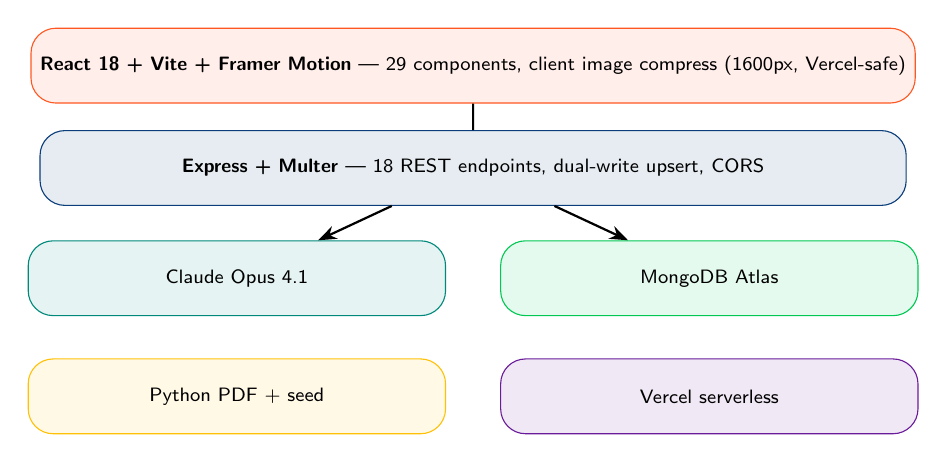
\begin{tikzpicture}[
    layer/.style={rectangle, rounded corners=9pt, draw=#1, fill=#1!10,
      minimum width=11cm, minimum height=0.95cm, align=center, font=\scriptsize},
    every node/.style={font=\scriptsize}]
    \node[layer=SSOrange] (fe) at (0,3.8)
      {\textbf{React 18 + Vite + Framer Motion} — 29 components, client image compress (1600px, Vercel-safe)};
    \node[layer=SSBlue] (be) at (0,2.5)
      {\textbf{Express + Multer} — 18 REST endpoints, dual-write upsert, CORS};
    \node[layer=SSTeal, minimum width=5.3cm] (ai) at (-3,1.1) {Claude Opus 4.1};
    \node[layer=SSGreen, minimum width=5.3cm] (db) at (3,1.1) {MongoDB Atlas};
    \node[layer=SSGold, minimum width=5.3cm] (py) at (-3,-0.4) {Python PDF + seed};
    \node[layer=SSPurple, minimum width=5.3cm] (vx) at (3,-0.4) {Vercel serverless};
    \draw[-{Stealth}, thick] (fe)--(be)--(ai);
    \draw[-{Stealth}, thick] (be)--(db);
  \end{tikzpicture}
\end{frame}

\begin{frame}{Dual-Write + Resilience — Enterprise-Grade Hackathon Code}
  \begin{columns}
    \column{0.5\textwidth}
    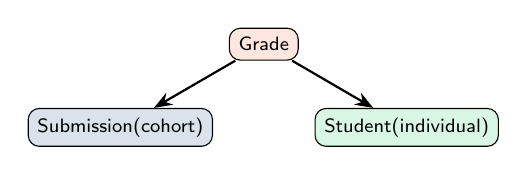
\begin{tikzpicture}[font=\scriptsize, node distance=0.45cm]
      \node[draw, fill=SSOrange!15, rounded corners] (g) {Grade};
      \node[draw, fill=SSBlue!15, rounded corners, below left=0.6cm and 0.2cm of g] (s) {Submission\\(cohort)};
      \node[draw, fill=SSGreen!15, rounded corners, below right=0.6cm and 0.2cm of g] (t) {Student\\(individual)};
      \draw[-{Stealth}, thick] (g)--(s);
      \draw[-{Stealth}, thick] (g)--(t);
    \end{tikzpicture}

    \column{0.48\textwidth}
    \footnotesize
    \begin{itemize}\setlength\itemsep{0.15em}
      \item \textbf{Low bandwidth:} compress to 3.5MB batches
      \item \textbf{Rate limits:} 429 exponential backoff
      \item \textbf{Serverless:} batch size 2 on Vercel
      \item \textbf{Partial failure:} allSettled per sheet
      \item \textbf{Unreadable:} manual review queue
    \end{itemize}
  \end{columns}

  \vspace{0.2cm}
  \smartdiagram[flow diagram:horizontal,font=\tiny]{
    Photos, Compress, Claude, JSON, DB, Dashboard
  }
\end{frame}

% ══════════════════════════════════════════════════════════════════
\section{Impact \& Policy}
% ══════════════════════════════════════════════════════════════════

\begin{frame}{NEP 2020 + SDG 4 Alignment}
  \begin{columns}[T]
    \column{0.5\textwidth}
    \begin{callout}[title={NEP 2020 — India}]{SSBlue}
      \footnotesize
      \begin{itemize}\setlength\itemsep{0.1em}
        \item \textbf{Formative assessment} — continuous, not summative-only
        \item \textbf{Competency-based} — our concept taxonomy
        \item \textbf{Mother tongue} — Hindi parent comms
        \item \textbf{Teacher empowerment} — reduce clerical load
      \end{itemize}
    \end{callout}

    \column{0.48\textwidth}
    \begin{callout}[title={UN SDG 4}]{SSGreen}
      \footnotesize
      \begin{itemize}\setlength\itemsep{0.1em}
        \item Quality education for all
        \item Equity — early weak-student detection
        \item Inclusion — mixed-ability classrooms
      \end{itemize}
    \end{callout}
  \end{columns}

  \vspace{0.25cm}
  \centering
  
\begin{tikzpicture}[font=\footnotesize]
    \node[draw=SSOrange, fill=SSOrange!12, rounded corners, minimum width=3.2cm, align=center] (a) {Assess better};
    \node[draw=SSBlue, fill=SSBlue!12, rounded corners, minimum width=3.2cm, align=center, right=0.4cm of a] (b) {Teach smarter};
    \node[draw=SSGreen, fill=SSGreen!12, rounded corners, minimum width=3.2cm, align=center, right=0.4cm of b] (c) {Learn faster};
    \draw[-{Stealth}, thick] (a)--(b)--(c);
  \end{tikzpicture}
\end{frame}

\begin{frame}{Unit Economics — Sustainable at Scale*}
  \begin{columns}
    \column{0.55\textwidth}
    \footnotesize
    \begin{tabular}{@{}lrr@{}}
      \toprule
      \textbf{Cost driver} & \textbf{Per 50-student test} & \textbf{Note} \\
      \midrule
      Claude API (vision) & $\sim$\$4.00 & Batch-optimized \\
      Infra (Vercel+Mongo) & $\sim$\$0.20 & Shared tenancy \\
      \textbf{Total} & \textbf{\$4.20} & \\
      \textbf{Per student} & \textbf{\$0.08} & \\
      School license (proj.) & Rs.~12/student/mo & 15 tests included \\
      Gross margin (proj.) & 62\% & At 500+ students/school \\
      \bottomrule
    \end{tabular}

    \column{0.42\textwidth}
    \begin{callout}[title={Flywheel}]{SSPurple}
      \footnotesize
      More tests $\rightarrow$ richer Error DNA $\rightarrow$ better risk predictions $\rightarrow$ higher teacher retention $\rightarrow$ more schools
    \end{callout}
  \end{columns}
  \tiny *Projections at Anthropic list pricing; edu discounts improve margin.
\end{frame}

\begin{frame}{Real-World Readiness Matrix}
  \footnotesize
  \renewcommand{\arraystretch}{1.3}
  \begin{tabular}{@{}lccc@{}}
    \toprule
    \textbf{Dimension} & \textbf{Now} & \textbf{Phase 2} & \textbf{Phase 3} \\
    \midrule
    Low connectivity & \pmark\ Compress + small batches & Offline queue & Edge cache \\
    Entry-level phones & \cmark\ SPA & PWA install & SMS fallback \\
    Hindi / regional & \pmark\ Parent AI msgs & Full UI i18n & Tamil, Marathi \\
    Offline grading & \xmark & Upload queue & On-device draft OCR \\
    Privacy / DPDP & \pmark\ Env keys & School tenancy & Consent flows \\
    WhatsApp integration & \xmark & Teacher bot & Parent auto-notify \\
    \bottomrule
  \end{tabular}

  \vspace{0.2cm}
  \badge{SSGreen}{India-first} Phone camera \textbullet{} No scanner \textbullet{} No LMS migration
\end{frame}

\begin{frame}{Responsible AI — Trust by Design}
  \begin{columns}[T]
    \column{0.5\textwidth}
    \footnotesize\cmark\ Teacher approves every intervention\\
    \cmark\ Parent messages = drafts, not auto-send\\
    \cmark\ Unreadable sheets $\rightarrow$ human review\\
    \cmark\ Auditable JSON logs\\
    \cmark\ Minimal PII (name on sheet only)

    \column{0.48\textwidth}
    \begin{callout}[title={Phase 2 Governance}]{SSSlate}
      \footnotesize
      Bias audits on handwriting styles \textbullet{}
      DPDP child consent \textbullet{}
      Explainability cards \textbullet{}
      School data isolation
    \end{callout}
  \end{columns}
\end{frame}

% ══════════════════════════════════════════════════════════════════
\section{Roadmap \& Vision}
% ══════════════════════════════════════════════════════════════════

\begin{frame}{Roadmap — Hackathon to National Scale}
  \centering
  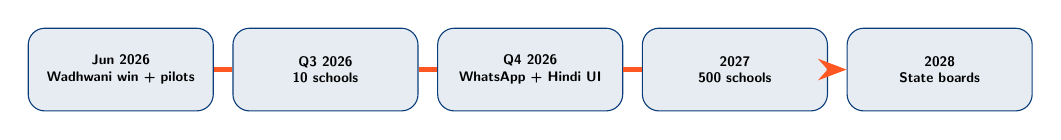
\begin{tikzpicture}[
    m/.style={rectangle, rounded corners=6pt, draw=SSBlue, fill=SSBlue!10,
      minimum width=2.35cm, minimum height=1.05cm, align=center, font=\tiny\bfseries}]
    \node[m] (a) at (0,0) {Jun 2026\\Wadhwani win + pilots};
    \node[m] (b) at (2.6,0) {Q3 2026\\10 schools};
    \node[m] (c) at (5.2,0) {Q4 2026\\WhatsApp + Hindi UI};
    \node[m] (d) at (7.8,0) {2027\\500 schools};
    \node[m] (e) at (10.4,0) {2028\\State boards};
    \draw[-{Stealth}, ultra thick, SSOrange] (a)--(b)--(c)--(d)--(e);
  \end{tikzpicture}

  \vspace{0.35cm}
  \begin{columns}[T]
    \column{0.33\textwidth}
    \textbf{Dependencies} \footnotesize
    \begin{itemize}\setlength\itemsep{0.08em}
      \item Wadhwani school intros
      \item API edu credits
      \item Champion teachers
    \end{itemize}
    \column{0.33\textwidth}
    \textbf{Risks} \footnotesize
    \begin{itemize}\setlength\itemsep{0.08em}
      \item OCR edge cases
      \item Cost at scale
      \item Adoption friction
    \end{itemize}
    \column{0.33\textwidth}
    \textbf{Out of scope} \footnotesize
    \begin{itemize}\setlength\itemsep{0.08em}
      \item Full LMS replace
      \item Board exam proctoring
    \end{itemize}
  \end{columns}
\end{frame}

\begin{frame}{Vision 2028 — India's Classroom Intelligence Standard}
  \centering
  \begin{tcolorbox}[enhanced,colback=SSBlue,colframe=SSBlue,coltext=white,
    arc=12pt,boxrule=0pt,width=0.92\textwidth, drop shadow]
    \Large\textbf{Every school test $\rightarrow$ same-day intelligence $\rightarrow$ every child seen}\\[0.35cm]
    \normalsize
    Shiksha Setu becomes the \textbf{default layer} between paper assessments and teaching action —\\
    like UPI for payments, but for \textbf{formative insight}.
  \end{tcolorbox}

  \vspace{0.4cm}
  \begin{columns}
    \column{0.33\textwidth}
    \metriccard{SSOrange}{0.95\columnwidth}{500}{Schools target}
    \column{0.33\textwidth}
    \metriccard{SSBlue}{0.95\columnwidth}{250K}{Students impacted}
    \column{0.33\textwidth}
    \metriccard{SSGreen}{0.95\columnwidth}{10M}{Tests analyzed / year}
  \end{columns}
  \tiny *Vision targets post-funding; methodology proven in hackathon prototype.
\end{frame}

% ══════════════════════════════════════════════════════════════════
\section{Demo \& Team}
% ══════════════════════════════════════════════════════════════════

\begin{frame}{60-Second Live Demo Script}
  \begin{enumerate}\setlength\itemsep{0.4em}
    \item[\badge{SSOrange}{\faIcon{upload}}] Upload 5 worksheets — show compress + progress
    \item[\badge{SSBlue}{\faIcon{list}}] Grading log — names, scores, concepts live
    \item[\badge{SSRed}{\faIcon{fire}}] Heatmap — ``Linear Equations'' URGENT
    \item[\badge{SSTeal}{\faIcon{user}}] Student profile — Error DNA + PDF download
    \item[\badge{SSGreen}{\faIcon{comment}}] Generate Hindi parent message — teacher reviews
  \end{enumerate}
  \vspace{0.15cm}
  \begin{callout}[title={\faIcon{shield-alt}\; Demo safety net}]{SSBlue}
    \footnotesize Pre-seeded MongoDB via \texttt{generate\_dataset.py} if Wi-Fi fails — judges still see full intelligence.
  \end{callout}
\end{frame}

\begin{frame}{Team Shiksha Setu}
  \begin{columns}[T]
    \column{0.55\textwidth}
    \footnotesize
    \renewcommand{\arraystretch}{1.5}
    \begin{tabular}{@{}p{2.5cm}p{4.5cm}@{}}
      \toprule
      \textbf{Role} & \textbf{Superpower} \\
      \midrule
      % CUSTOMIZE
      Full-Stack Lead & Shipped 29 UI modules + 18 APIs \\
      AI Engineer & 3 Claude pipelines + eval framework \\
      Product / EdTech & Teacher workflows + Wadhwani fit \\
      Data / Platform & Vercel deploy + dataset + PDFs \\
      \bottomrule
    \end{tabular}

    \column{0.42\textwidth}
    \smartdiagram[constellation diagram,font=\tiny]{
      React, Node, Claude, MongoDB, Python, Bharat EdTech
    }
    \vspace{0.15cm}
    \badge{SSOrange}{Add photos \& names before pitch}
  \end{columns}
\end{frame}

\begin{frame}{The Ask — Partner With Us to Scale}
  \begin{columns}
    \column{0.48\textwidth}
    \begin{callout}[title={What we need from Wadhwani}]{SSBlue}
      \footnotesize
      \begin{itemize}\setlength\itemsep{0.12em}
        \item \textbf{Pilot intros} — 2 urban + 2 semi-urban schools
        \item \textbf{Mentorship} — India ed-AI ethics \& scale
        \item \textbf{API credits} — 8-week validation study
        \item \textbf{Visibility} — Wadhwani portfolio showcase
      \end{itemize}
    \end{callout}

    \column{0.48\textwidth}
    \begin{callout}[title={What you get}]{SSGreen}
      \footnotesize
      \begin{itemize}\setlength\itemsep{0.12em}
        \item Production-ready prototype \textbf{today}
        \item Direct challenge alignment
        \item Differentiated AI (not wrapper)
        \item Path to 250K students by 2028*
      \end{itemize}
    \end{callout}
  \end{columns}

  \vspace{0.3cm}
  \centering
  \begin{tcolorbox}[enhanced,colback=SSGradA,colframe=SSGradA,coltext=white,
    halign=center,width=0.9\textwidth,arc=12pt,boxrule=0pt,drop shadow]
    {\LARGE\bfseries शिक्षा सेतु — Shiksha Setu}\\[0.15cm]
    {\large\textbf{We don't grade faster. We teach smarter.}}\\[0.1cm]
    Wadhwani AI Hackathon 2026 — Thank you!
  \end{tcolorbox}
\end{frame}

% ══════════════════════════════════════════════════════════════════
\appendix
\section*{Appendix}

\begin{frame}{Appendix — Innovation Glossary}
  \footnotesize
  \begin{tabular}{@{}lp{8.5cm}@{}}
    \toprule
    \textbf{Term} & \textbf{Meaning} \\
    \midrule
    Error DNA & Persistent misconception store per student \\
    Setu-Buckets™ & Adaptive percentile thresholds for heatmap \\
    Setu-Comms™ & Bilingual AI parent message generator \\
    SETU-EDU JSON & Structured schema for classroom AI interop (roadmap) \\
    Dual-Write & Submission (cohort) + Student (individual) sync \\
    \bottomrule
  \end{tabular}
\end{frame}

\begin{frame}{Appendix — API Reference}
  \tiny
  \begin{multicols}{2}
  \textbf{Grading}\\ \texttt{POST /evaluate}\\
  \texttt{GET /heatmap-report}\\
  \texttt{GET /recommendations}\\
  \texttt{GET /at-risk-students}\\
  \texttt{GET /peer-benchmarking}\\
  \texttt{GET /practice-test/:concept}

  \columnbreak
  \textbf{Students}\\ \texttt{POST /:id/grade}\\
  \texttt{POST /parent-message}\\
  \texttt{POST /risk-assessment}\\
  \texttt{GET /class-misconceptions}\\
  \texttt{GET /tests/:id/replay}
  \end{multicols}
\end{frame}

% ══════════════════════════════════════════════════════════════════
\begingroup
\setbeamertemplate{background}{}
\setbeamertemplate{footline}{}
\begin{frame}[plain,noframenumbering]
  \begin{tikzpicture}[remember picture,overlay]
    \shade[bottom color=SSGradA, top color=SSBlueLight]
      (current page.south west) rectangle (current page.north east);
    \foreach \i in {1,...,8}
      \draw[white, opacity=0.05] ([xshift=\i*1.7cm,yshift=0.5cm]current page.south west)
        -- ++(0,8);
    \node[white, align=center] at (current page.center) {
      {\fontsize{40}{44}\selectfont\bfseries Questions?}\\[0.7cm]
      {\LARGE Shiksha Setu — शिक्षा सेतु}\\[0.4cm]
      {\large From paper piles to precision teaching — for every child.}\\[0.9cm]
      {\normalsize\faIcon{github}\quad github.com/YOUR-REPO \quad
       \faIcon{envelope}\quad team@shikshasetu.in}\\[0.35cm]
      {\footnotesize\color{white!70} Live demo ready on stage \quad\textbullet\quad Backup dataset loaded}
    };
  \end{tikzpicture}
\end{frame}
\endgroup

\end{document}
